\chapter{Case of study} \label{case}

\section{Experimental settings} 

In this particular experimental scenario, the basic guidelines 
proposed in Adomavicius \cite{adomavicius2011context} are followed,  
and they are briefly explained next. 
\begin{itemize} 
\item \textbf{Hypothesis:} before running the experiment we must form
an \textit{hypothesis}. It is important to be concise and restrictive
about this hypothesis, and design an experiment that tests the
hypothesis. For example, an hypothesis can be that  \textbf{algorithm
A} predicts better user ratings than  \textbf{algorithm B}.  In that
case, the experiment should test the prediction accuracy, and not
other factors.
\item \textbf{Controlling variables:} when comparing a few candidate
algorithms on a certain hypothesis, it is important that all
\textit{variables} that are not tested will stay fixed. For example,
suppose that we wish to compare the prediction accuracy of movie
ratings of  \textbf{algorithm A} and \textbf{algorithm B}, that both
use different collaborative filtering models.
\item \textbf{Generalization power:} when drawing conclusions from
experiments, we may desire that our conclusions generalize beyond the
immediate context of the experiments. When choosing an algorithm for a
real application, we may want our conclusions to hold on the deployed
system, and generalize beyond our experimental data set. Similarly,
when developing new algorithms, we want our conclusions to hold beyond
the scope of the specific application or data set that we experimented
with. It is important to understand the properties of the various data
sets that are used. Generally speaking, \textit{the more diverse the
data used, the more it can generalize the results}.
\end{itemize} 

\subsection{Off-line experiments} 

An off-line experiment is performed using a pre-collected dataset
of users choosing or ratings. Using this dataset tries to simulate
the behavior of users that interact with a recommender system. In
doing so, it assume that the user behavior when the data was collected
will be similar enough to the user behavior when the recommender
system is deployed, so that we can make reliable decisions based on
the simulation.  Off-line experiments are attractive because they
\textit{require no interaction with real users}, and thus it allows to compare
a wide range of candidate algorithms at a low cost. \\ The downside is
that it can answer a very narrow set of questions, typically questions
about the prediction of an algorithm. The goal of the off-line
experiments is to filter out inappropriate  approaches, leaving a
relatively small set of alternatives algorithms for subsequently to be
tested for the more costly user studies or on-line 
experiments\cite{adomavicius2011context}.\\ 
The next section shows a comprehensive description of the 
experimental setup for experiments, as well as results obtained 
in the experiments.
Each method was tested using contextual datasets in the domain. 
Results are showed in order to  compare the performance of the 
algorithms in the method. 
%% Haz un puente, dices que vaz a hacer ciertos experimentos
%% menciona aquí que lo que sigue es el setup de tus parte experimental.
%% Menciona brevemente los experimentos o datrasets, Restaurants, MovieLens,
%% Filmtrust and InCarMusic, TripAdvisor
%\section{Experiments} 
%% Esto creo que ya se había dicho,
%% o debe ir en Method
\section{Restaurants recommendations} 

Previous the implementation of context-aware recommender system  
some experiments were done to test the behaviour of algorithms 
and the performance in the proposed method. 
For the experiment the proposed hypothesis is \textit{The accuracy of 
recommendations is improved using the context in the 
recommendation process}. To validate the hypothesis the next test  
was realized. \\
A first experiment\cite{ramirez2013restaurant}  presents a  
contextual recommender system using the post-filtering approach,  
collaborative filtering is used to find relevant  restaurants for users.  
Later, the Top-N list is obtained and the restaurants are adjusted to 
make ranking of restaurants  in the current context. Post-filtering is
based on the average  of ratings in a specific context, so prediction
is made with: 1) \textit{the average} that a restaurant has in the
current context (that is the  mean of user ratings) and 2) 
\textit{the rating} predicted by the collaborative filtering algorithm. 
The top-N list contains the restaurants with highest predictions, 
so each restaurant is adjusted for the user's context and listed in 
contextual recommendations; the process is depicted in figure
\ref{fig:postfiltering}.
\begin{figure*}
\centering
\captionsetup{font=footnotesize}
\setlength\fboxsep{0pt}
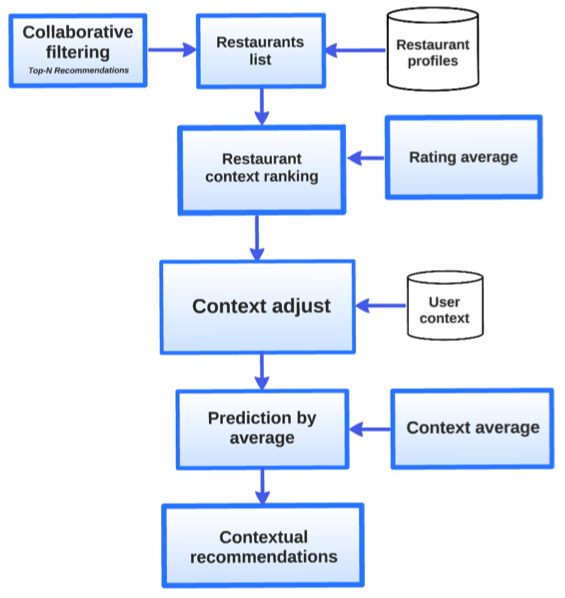
\includegraphics[width=0.50\textwidth]{img/posfil.png}
\caption{The post-filtering approach for Tijuana restaurants.}
\label{fig:postfiltering}     
\end{figure*}
%% Bien, empieza aquí:
%Algo como
%In order to validate the proposed approach described in section XXX, data about restaurant
The evaluation of the proposed approach is using data 
about restaurant preferences of users in different contexts. 
The study subjects were students  with a major in engineering,  
master's program and professors of the Tijuana Institute of
Technology. A total of \textit{50 users} answered a questionnaire; the
questions were about their preferences for nearby restaurants and the
technology most often used by them. The \textit{questionnaire} consisted 
of \textit{8 questions} and also they were asked to rate any number 
of restaurants from a list of 40 restaurants.
Each of the restaurants chosen, was rated 6 times one per proposed 
context, a matrix rating with \textit{1,422 ratings} was collected. The
questions are shown in table \ref{tab:questions}. The reason for allowing
users to chose what restaurants to rate it to give them the same liberty
that they have when visiting a web or mobile application. 
\begin{table}
\small
\captionsetup{font=footnotesize}
\caption{Questionnaire applied to collect contextual dataset.}
\label{tab:questions} 
\centering
\small
\begin{tabular}{p{7cm} p{5cm} }
\hline\noalign{\smallskip}
Question & Answers \\
\noalign{\smallskip}\hline\noalign{\smallskip}
\small{1.What is your occupation?} & \small{1. Student 2.Employee} \\ \hline  
\small{2.According your priority, order by importance the features 
you consider when you choose to visit a restaurant.} & 
\small{1.Installation/decoration 2.Prices 3.Service 4.Dishes
5.Atmosphere 6.Location} \\ \hline  
\small{3.What are the devices that you used
utilizes?} & \small{1.Smartphone 2.Tablet 3.Laptop 4.PC} \\ \hline   
\small{4.What Operating System do you used?} & 
\small{1.Android 2.Windows 3.iOS 4.Symbian 5.Blackberry 6.Other}
\\ \hline  
\small{5.Did you use an application to search restaurants in Tijuana?} &
\small{1.Yes 2.No 3.Which one?} \\ \hline   
\small{6.Would you like to use an application of
recommender systems of Tijuana?} & \small{1.Yes 2.No} \\ \hline  
\small{7.Please, rates your favorites restaurants(without context).} & 
\small{Restaurant list} \\ \hline
\small{8.Please, rates your favorites restaurants in contextual situations.} & 
\small{Restaurant list} \\
\noalign{\smallskip}\hline
\end{tabular}
\end{table}
The user's answers from question 1 to question 6 are represented in
the figure \ref{fig:cakeschart}. \textit{Figure \ref{fig:cakeschart}a}
represents the percentage of surveyed students and teachers;
\textit{figure \ref{fig:cakeschart}b}  the percentage of the element
that users consider the most important to visit a restaurant;
\textit{figure \ref{fig:cakeschart}c} represents the preferences of
devices when are using Internet for restaurant recommendations;
\textit{figure \ref{fig:cakeschart}d} represents the percentage of
operating system that often used, \textit{figure
\ref{fig:cakeschart}e} shows the percentage of users that use the
Internet to search restaurants in Tijuana; and \textit{figure
\ref{fig:cakeschart}f}, shows the percentage of users that would like
using a restaurant recommender system of Tijuana.
\begin{figure*}
\captionsetup{justification=centering,margin=2cm,font=footnotesize}
\centering
\setlength\fboxsep{0pt}
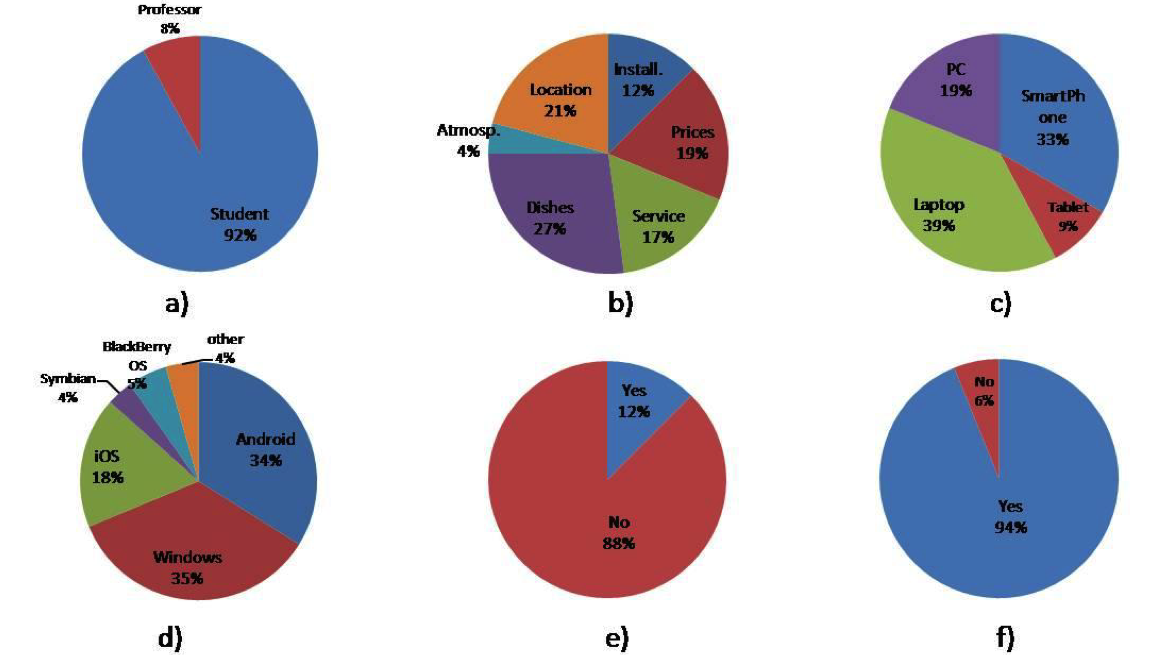
\includegraphics[width=0.8\textwidth]{img/cakes.png}
\caption{The chart cakes show the users preferences for questions from 1 to 6.}
\label{fig:cakeschart}     
\end{figure*}
For questions 7 and 8 only the top-ten restaurants are shown,
without/with the contextual situation. In figure \ref{fig:barschart}a,
the favorite restaurant is \textbf{Daruma}(178 votes),  whereas in
figure \ref{fig:barschart}b, \textbf{Daruma} does not appear in the
top-ten. When considering the context \textit{midweek}, the favorite
restaurant was \textbf{Carl's Jr.}, which appears in both graphs; this
restaurant was also the most voted in the different contexts.
\begin{figure*}
\captionsetup{justification=centering,margin=2cm,font=footnotesize}
\centering
\setlength\fboxsep{0pt}
%\setlength\fboxrule{0.7pt}
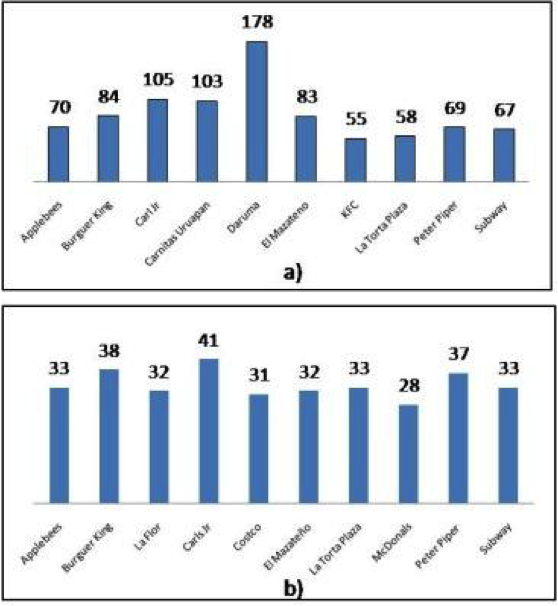
\includegraphics[width=0.55\textwidth]{img/bars.png}
\caption{The chart shows the users preferences for questions 7 and 8.}
\label{fig:barschart}     
\end{figure*}
Contextual recommendations of post-filtering approach depends of
context \textit{midweek} or \textit{weekend}, which is the day when
the restaurants were rated. Subsequently, the result of the query is
refined according to the user context; the 6 contexts mentioned
correspond to combinations of contextual factors shown in table
\ref{tab:contextstijuana}.
\begin{table}
\small
\captionsetup{font=footnotesize}
\caption{Contextual factors considered in the questionnaire.}
\label{tab:contextstijuana} 
\centering
\begin{tabular}{p{2.5cm} p{7cm} }
\hline\noalign{\smallskip}
Contextual Factor & Context \\
\noalign{\smallskip}\hline\noalign{\smallskip}
\small{Day} & \small{1.Midweek(Monday, Thuesday,Wednesday and Thursday)
2.Weekend(Friday,Saturday and Sunday)}  \\ \hline 
\small{Place} & \small{1.School 2. Home 3.Work} \\ 
\noalign{\smallskip}\hline
\end{tabular}
\end{table}
The  mean absolute error obtained was \textbf{0.5859} 
in contextual recommendations. 
The observation for this result is that using a small
dataset the performance of the method proposed is limited, the cold-start 
problem affects the accuracy because of the data scarcity.

\section{Hotels recommendations} 

A second experiment using TripAdvisor dataset was used. 
For this case, the proposed method consists of three algorithms 
to recommend:  \textit{fuzzy inference system}, \textit{collaborative 
filtering} and \textit{content-based}. Each one uses the ratings 
matrix to get recommendations.\\    
The contextual recommender system uses  \textit{post-filtering}
approach\cite{adomavicius2011context} for adjust recommendations in
context such as restaurants. The recommendation by popularity is 
through the fuzzy inference system depicted in figure \ref{fig:fis}, 
the fuzzy inference
system contains the variables that are involved in the process to
recommend in a human interaction, this process is the same that the
recommender system does. \\The output represents how matter each item
into the users community, i.e. if it is a popular item between users. \\
The dataset used to evaluate the algorithm was TripAdvisor in two
versions downloaded\cite{linkzeng}, this datasets was used in
\cite{zheng2014context} and \cite{zheng2012differential} to  evaluate the
performance of context-aware recommender systems. \\The first
dataset contains 4669 contextual ratings, 1202 users and 1890 hotels;
the second dataset contains 14175 contextual ratings, 2731 users and
2269 hotels. Data were collected of reviews online in tripadvisor.com.
There is only one context: \textit{type of trip} (family, friends, bussines,
romantic and relax).\\ 
The FIS has Gaussians membership functions and are depicted in figure
\ref{fig:mffis}.
\begin{figure}[ht!]
   \captionsetup{font=footnotesize}
   \centering
   %%----primera subfigura----
   \subfloat[]{
        \label{fig:1a}
        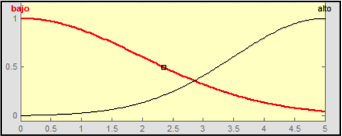
\includegraphics[width=0.42\textwidth]{img/ratingaverage.png}}
   \hspace{0.1\linewidth}
   %%----segunda subfigura----
   \subfloat[]{
        \label{fig:1b} 
        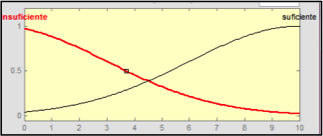
\includegraphics[width=0.42\textwidth]{img/userparticipation.png}}\\[20pt]
   %%----tercera subfigura----
    \subfloat[]{
        \label{fig:1c} 
        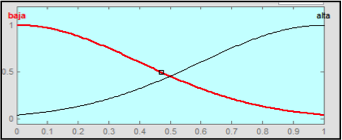
\includegraphics[width=0.42\textwidth]{img/recommendation.png}}
   \caption{Gaussian Membership functions in the input are: a) RatingAverage, 
   b) UserParticipation, and an output: c) Recommendation.}
   \label{fig:mffis} 
\end{figure}
The fuzzy inference system uses fuzzy rules to infer the inputs and 
output(a crisp value) that represents the weight of the recommendation. 
The rules are following: 
\begin{enumerate}
\item \textit{If \textbf{RatingAverage} is low and 
\textbf{UserParticipation} is insufficient then \textbf{recommendation} is low.}
\item \textit{If \textbf{RatingAverage} is low and 
\textbf{UserParticipation} is sufficient then \textbf{recommendation} is high.}
\item \textit{If \textbf{RatingAverage} is high and 
\textbf{UserParticipation} is insufficient then \textbf{recommendation} is low.}
\item \textit{If \textbf{RatingAverage} is high and 
\textbf{UserParticipation} is sufficient then \textbf{recommendation} is high.}
\end{enumerate}
\begin{figure*}
\captionsetup{justification=centering,margin=2cm,font=footnotesize}
\centering
\setlength\fboxsep{0pt}
\setlength\fboxrule{0.7pt}
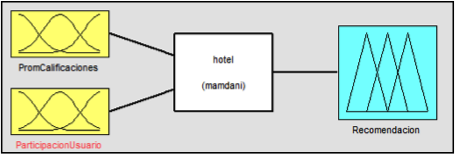
\includegraphics[width=0.75\textwidth]{img/fis.png}
\caption{Fuzzy Inference System.}
\label{fig:fis}   
\end{figure*}
Content-based uses cosine similarity to compare the binary
vectors representing the profile of each item, thereby obtaining a
numerical value that determines similarity, based on a threshold. \\   
In other words, it makes a comparison of profiles of each item to
determine the most similar to items the user has rated with highest
score, context-aware recommender system proposed has a scale 
from 1 to 5. 
\begin{table}[htb]
\small
\centering
\captionsetup{font=footnotesize}
\caption{Example of contextual ratings in the user profile.}
\label{tab:2}
\small
\begin{tabular}{lll}
\hline
\multicolumn{3}{c}{\textbf{User profile}} \\ \hline
Item & Rating & Context \\ \hline
La Casa del Mole & 5.0 & Midweek \\ 
Daruma           & 4.0 & Weekend \\ 
Daruma           & 5.0 & Midweek \\ 
Carl's Jr.       & 3.0 & Weekend \\ \hline
\end{tabular}
\end{table}
In the next step the outputs of every recommender algorithm is
represented by a list of recommended items. Subsequently applies the
context filter and context-aware recommender system gets the final
contextual recommendations. Context-aware
recommender system identifies contextual data of the user profile (see
table \ref{tab:2}), and compares recommended items to filter those
items that are adjusted to the user context. 
The context filtering is the last step before to get the recommended
items. The schema of architecture for context-aware recommender system
is depicted in figure \ref{fig:architecture}.
\begin{figure*}
\captionsetup{font=footnotesize}
%\captionsetup{justification=centering,margin=2cm}
\centering
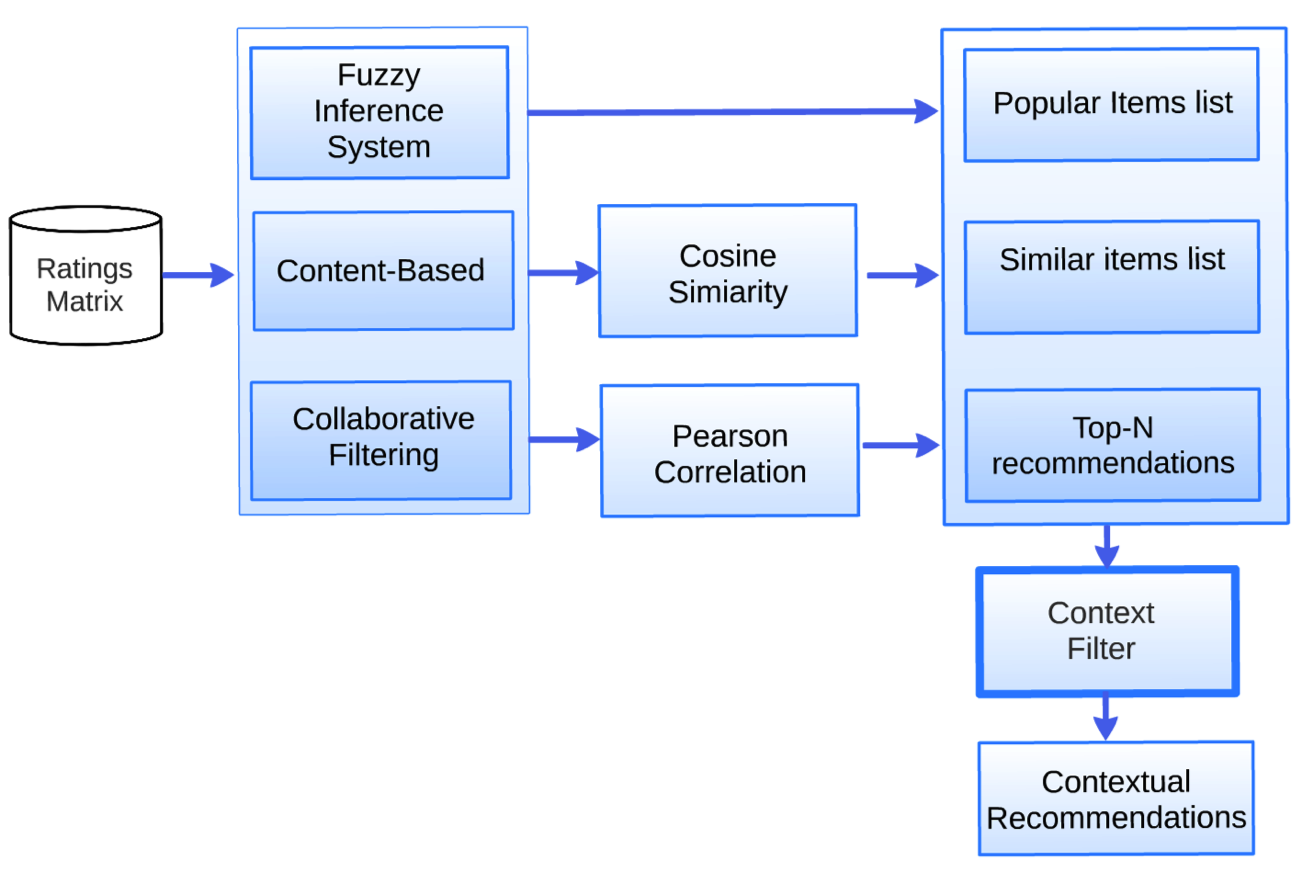
\includegraphics[width=0.80\textwidth]{img/archit-ta.png}
\caption{Recommender system methodology.}
\label{fig:architecture}   
\end{figure*}
Two experiments were performed using TripAdvisor dataset, table
\ref{tab:3} describes the data sets and the scarcity percentage of the
specified data. Scarcity of 99\% mean that there are problems to
recommend items because the information is not enought to get 
good recommendations.\\  By other side, in table \ref{tab:4} the comparison
shows that the algorithm has a acceptable performance, i.e., the error
falls into the range of results obtained with others algorithms. Then,
contextual recommendations were evaluated with the Root Mean Square
Error in order to compare the results with context relaxation
algorithm\cite{zheng2012differential} that is evaluated with the same
dataset.
\begin{table}
\centering
\small
\captionsetup{font=footnotesize}
\caption{Datasets description.}
\label{tab:3}      
\begin{tabular}{lllll}
\hline\noalign{\smallskip}
Dataset & Users & Items & Ratings & Scarcity (percent) \\
\noalign{\smallskip}\hline\noalign{\smallskip}
TripAdvisor v1 & 1202 & 1890 & 4669 & 99.79 \\
TripAdvisor v2 & 2731 & 2269 & 14175 & 99.77 \\
\noalign{\smallskip}\hline
\end{tabular}
\end{table}
\begin{table}
\centering
\small
\captionsetup{font=footnotesize}
\caption{Comparison of RMSE.}
\label{tab:4}  
\small   
\begin{tabular}{lll}
\hline\noalign{\smallskip}
Dataset & Algorithm & RMSE \\
\noalign{\smallskip}\hline\noalign{\smallskip}
TripAdvisor v2 & FC + Post-filtering  & 0.504  \\
               & FC          & 0.994  \\
               & Pre-filtering + Relaxation & 0.985  \\
\noalign{\smallskip}\hline
\end{tabular}
\end{table}
The cosine similarity plays an important role in content-based because
if similarity value among items is high, the recommendations will
improve the degree of user satisfaction. \\ This is observed when
calculating the similarity average in each dataset as shown in table
\ref{tab:5}.
\begin{table}
\centering
\small
\captionsetup{font=footnotesize}
\caption{Level of similarity among items in datasets. }
\label{tab:5}      
\begin{tabular}{lll}
\hline\noalign{\smallskip}
Dataset  & Similarity  & Avg.votes per user. \\
\noalign{\smallskip}\hline\noalign{\smallskip}
TripAdvisor v1 & 0.448  & 5  \\
TripAdvisor v2 & 0.508  & 8  \\
\noalign{\smallskip}\hline
\end{tabular}
\end{table}
FIS can provides a list of popular items for each dataset,
recommendations through averages are obtained, and recommendations are
conditioned to show it when the collaborative filtering and content-
based are not delivering recommendations because of data scarcity.\\ 
However, the majority of popular items of dataset were rated in contexts: 
\textit{romantic, family and bussines}, that means that the dataset has
biases.\\  In this experiment  the context-aware recommender system
proposed involves post-filtering for contextual
recommendations. The structure of the datasets facilitated the
evaluation of recommendations although the rating matrix has been
scarce in both cases. Anyway, information of items and users was used
to test the system and a good performance of the system was done.\\   
With respect the performance, post-filtering allows to select relevant
items that are adjusted into the context, indeed, post-filtering and
implementation of different recommendation techniques the system has
suitable performance and the datasets help the processes performed.

\section{Context-aware recommender system application} 

For the development of the recommender system was used python
language.  Django Framework and other dependencies were used in order
to complete the system functionality.





